\subsection*{2.1}
%    1. Build a common-source MOS amplifier as shown below using BS170 transistor.
%Element values: R1 = R2 = 100 k, R3 = R4 = 470 , RL = 1 k, C1 = 1 µF, C2 = 100 µF,
%C3 = 10 µF. Use VDD = 15 V.
A common-source MOS amplifier as shown in figure 3 below using BS170 transistor and the components shown in table 2.

\begin{table}[htbp]
   \centering
   \caption{Components}
     \begin{tabular}{rrrrrrrrrr}
     Component   & $R_1$       & $R_2$       & $R_3$       & $R_4$       & $R_L$       & $C_1$       & $C_2$       & $C_3$       & $V_{DD}$ \\
     Theoretical & $100 \ k \Omega$ & $100 \ k \Omega$ & $470 \ \Omega$ & $470 \ \Omega$ & $1.00 \ k \Omega$ & $1.000 \ \mu F$ & $100.0 \ \mu F$ & $10.00 \ \mu F$ & $15.000 \ V$ \\
     Measured    & $94 \ k \Omega$ & $98.5 \ k \Omega$ & $462 \ \Omega$ & $462 \ \Omega$ & $1.05 \ k \Omega$ & $1.015 \ \mu F$ & $98.4 \ \mu F$ & $10.09 \ \mu F$ & $15.373 \ V$ \\
     \end{tabular}%
   \label{tab:addlabel}%
\end{table}%


    \begin{figure}[h!]
        \centering
        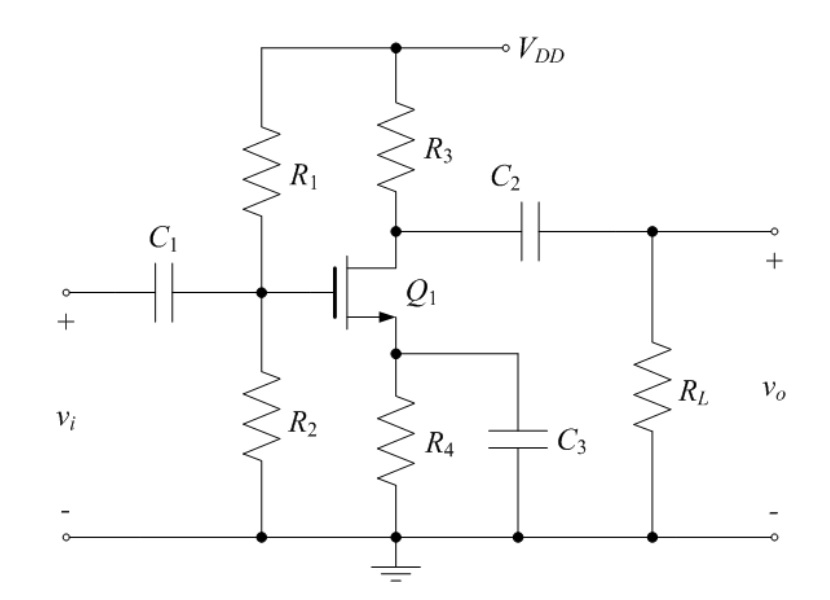
\includegraphics[width=6cm]{circuit_task_2.jpg}
        \captionof{figure}{Circuit built in task 2}
    \end{figure}


\pagebreak
\subsection*{2.2}

%2. Use Bode Analyzer to measure the AC characteristic of the amplifier in the frequency
%range 10 Hz to 50 kHz. Use 10 steps per decade and input signal amplitude of 50 mV.
%Find the lower 3dB frequency of the circuit.

A Bode Analyzer was used to measure the AC characteristic of the amplifier in the frequency range 10 Hz to 50 kHz using 10 steps per decade and input signal amplitude of 50 mV. The result of this analysis is shown in figure 4.

    \begin{figure}[h!]
        \centering
        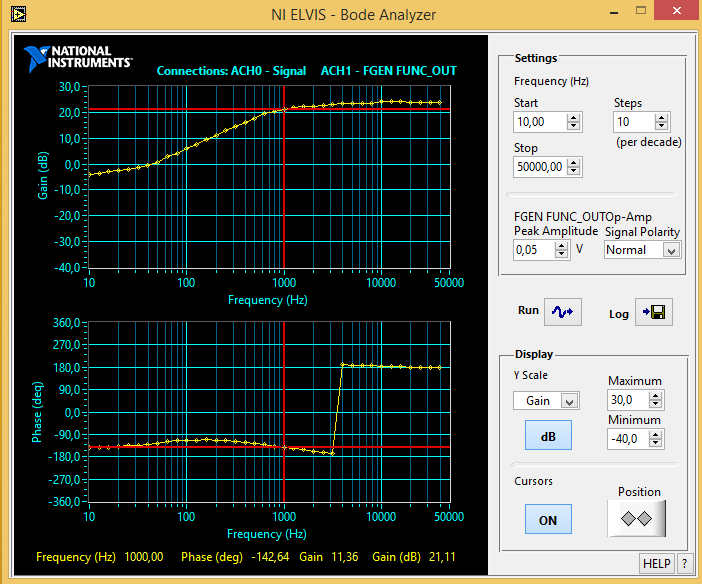
\includegraphics[width=8cm]{Task2-2-1.png}
        \captionof{figure}{AC characteristics of the amplifier showing the lower 3dB frequency of the circuit}
    \end{figure}

    \begin{figure}[h!]
        \centering
        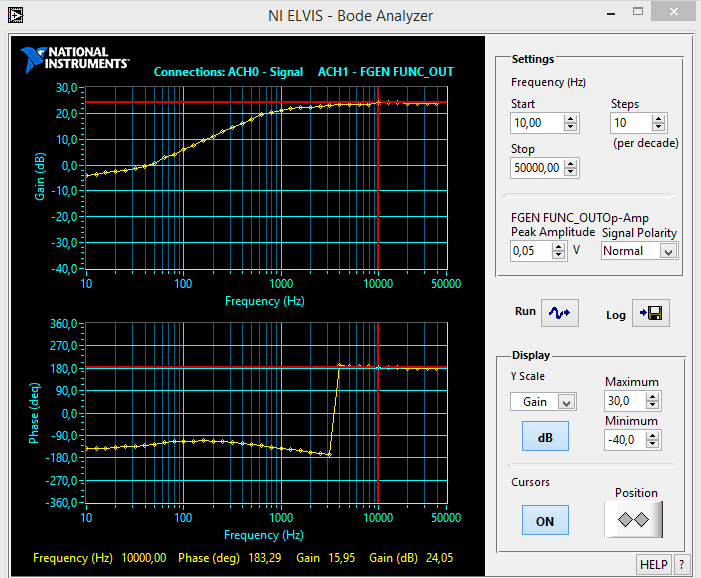
\includegraphics[width=8cm]{Task2.png}
        \captionof{figure}{AC characteristics of the amplifier showing the midband gain of the circuit}
    \end{figure}

From figure 4, the 3dB frequency can be seen as 1 kHz and from figure 5 the midband gain $$A_1 = 24.05 dB = 10^{24.05/20} \frac{V}{V} = 15.94 \frac{V}{V}$$


\pagebreak
\subsection*{2.3}
%3. Determine the following parameters of the circuit (at the frequency 1 kHz): voltage gain,
%input resistance, output resistance. Input signal amplitude should be small, e.g., 50 mV.
%Observe and store the input and output signal waveforms using oscilloscope.

    \begin{figure}[h!]
        \centering
        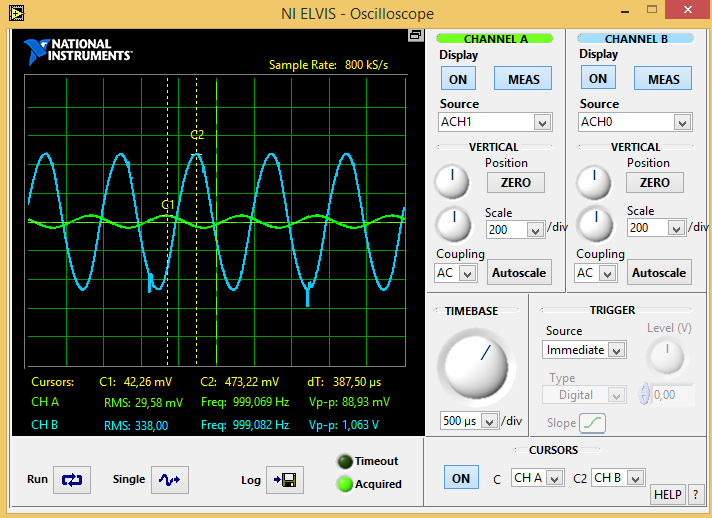
\includegraphics[width=8cm]{Task2-3.png}
        \captionof{figure}{Oscilloscope plot of the circuit in figure 3}% without $R_{s}$}
    \end{figure}

	Figure 6 shows the oscilloscope plot of the circuit in figure 3. The green wave is the input voltage and the blue wave is the output voltage. By taking the amplitude of blue wave and dividing by amplitude of the green wave gives the midband gain.

	$$ A_{M1} = \frac{473.22 mV}{42.26 mV} = 11.19 \frac{V}{V} $$

\pagebreak

    \begin{figure}[h!]
        \centering
        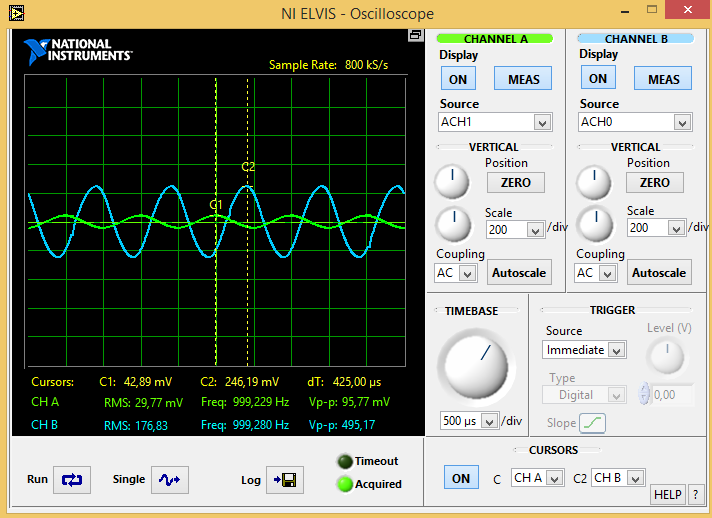
\includegraphics[width=8cm]{Task2-3-Rin.png}
        \captionof{figure}{Oscilloscope plot of the circuit in figure 3 after adding $R_s$}
    \end{figure}

	Figure 7 shows the oscilloscope plot of the circuit in figure 3 with an added $R_{s}$. By adding $R_{s}$ to the circuit, the new midband gain can be determined.

	$$ A_{M2} = \frac{245.19 mV}{42.89 mV} = 5.72 $$

	The midband gain from circuit without $R_{s}$ and with $R_{s}$ are used to find the $R_{in}$. The formula for midband gain with $R_{s}$ is:  

	$$A_{M2} = A_{M1} \cdot \frac{R_{in}}{R_{in} + R_{s}} \rightarrow R_{in} = \frac{R_{s}}{\frac{A_{M1}}{A_{M2}}-1}  $$

	$$  R_{in} = \frac{46.4 k \Omega }{\frac{11.19}{5.72}-1} = 48.52 k \Omega$$ 

\pagebreak

	\begin{figure}[h!]
        \centering
        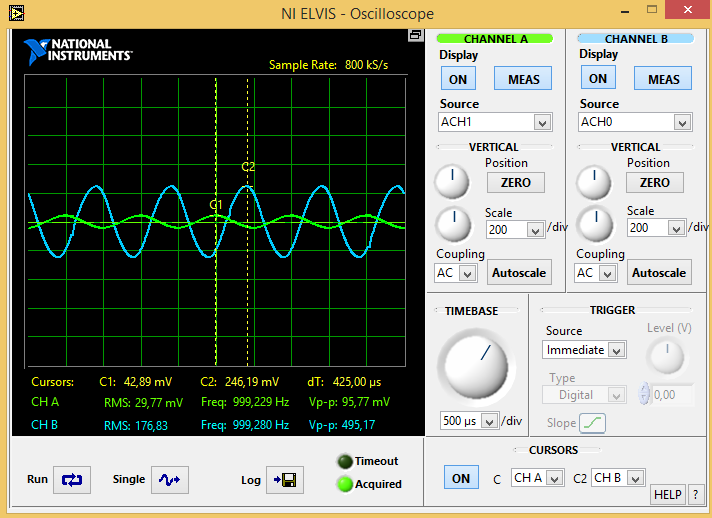
\includegraphics[width=8cm]{Task2-3-Rin.png}
        \captionof{figure}{Oscilloscope plot of the circuit in figure 3 without $R_L$}
    \end{figure}

	Figure 8 shows the oscilloscope plot of the circuit in figure 3 without $R_{L}$. By removing the load resistor and finding the midband gain from the amplitude of the waves in figure 8.


	$$ A_{M3} = \frac{681.05 mV}{42,29 mV} = 16.1 \frac{V}{V} $$

	By using the midband gain from the circuit with $R_{L}$ and without $R_{L}$ to find the $R_{out}$. The formula for midband gain without $R_{L}$ is:


	$$ A_{M3} = A_{M1} \cdot \frac{R_{L}}{R_{L} + R_{out}} \rightarrow R_{out} = R_{L} \cdot (\frac{A_{3}}{A_{1}}-1) = 460.72 \frac{V}{V}$$

\pagebreak




\subsection*{2.4}
% 4. Using the transistor parameters obtained in Task 1, determine the values of gain,
%input/output resistance and the lower 3dB frequency theoretically compare them to the
%values obtained experimentally.

The transistor parameters obtained in Task 1 were used to determine the values of gain, input/output resistance and the lower 3dB frequency theoretically. Calculations can be seen in appendix I.\\

\begin{table}[htbp]
    \centering
        \begin{tabular}{ c | c | c }
        \hline
        Circuit Parameters     &   Theory                  & Simulation \\
        \hline
        Midband voltage gain    &   25.68 dB			    &   24.05 dB\\
        Lower 3dB frequency     &   979.9 Hz                &   1000 Hz\\
        Input Resistance        &   48.1 k$\Omega$           &   48.5 k$\Omega$\\
        Output Resistance       &   462 k$\Omega$            &   460.7 k$\Omega$\\
        \end{tabular}%
    \caption{Theoretical parameters compared to experimental parameters.}
    \label{tab:addlabel}%
\end{table}%

Parameters obtained by experimentally agree with those determined theoretically. Derivation of theoretical values is in appendix 1.

The theoretical data determined by calculation was close to the measured data. But the difference in the midband gain and the Lower 3dB frequency is caused by the instruments used (the elvis), that is, when determining the threshold voltage. It would have been better to be able take more accurate measurements but the Elvis didn't support more accuracy. When the threshold voltage is off by a small factor the  transconductance factor (k) varies very quickly by multiples of itself. 


\pagebreak
\subsection*{Appendix 1}
\begin{figure}[h!]
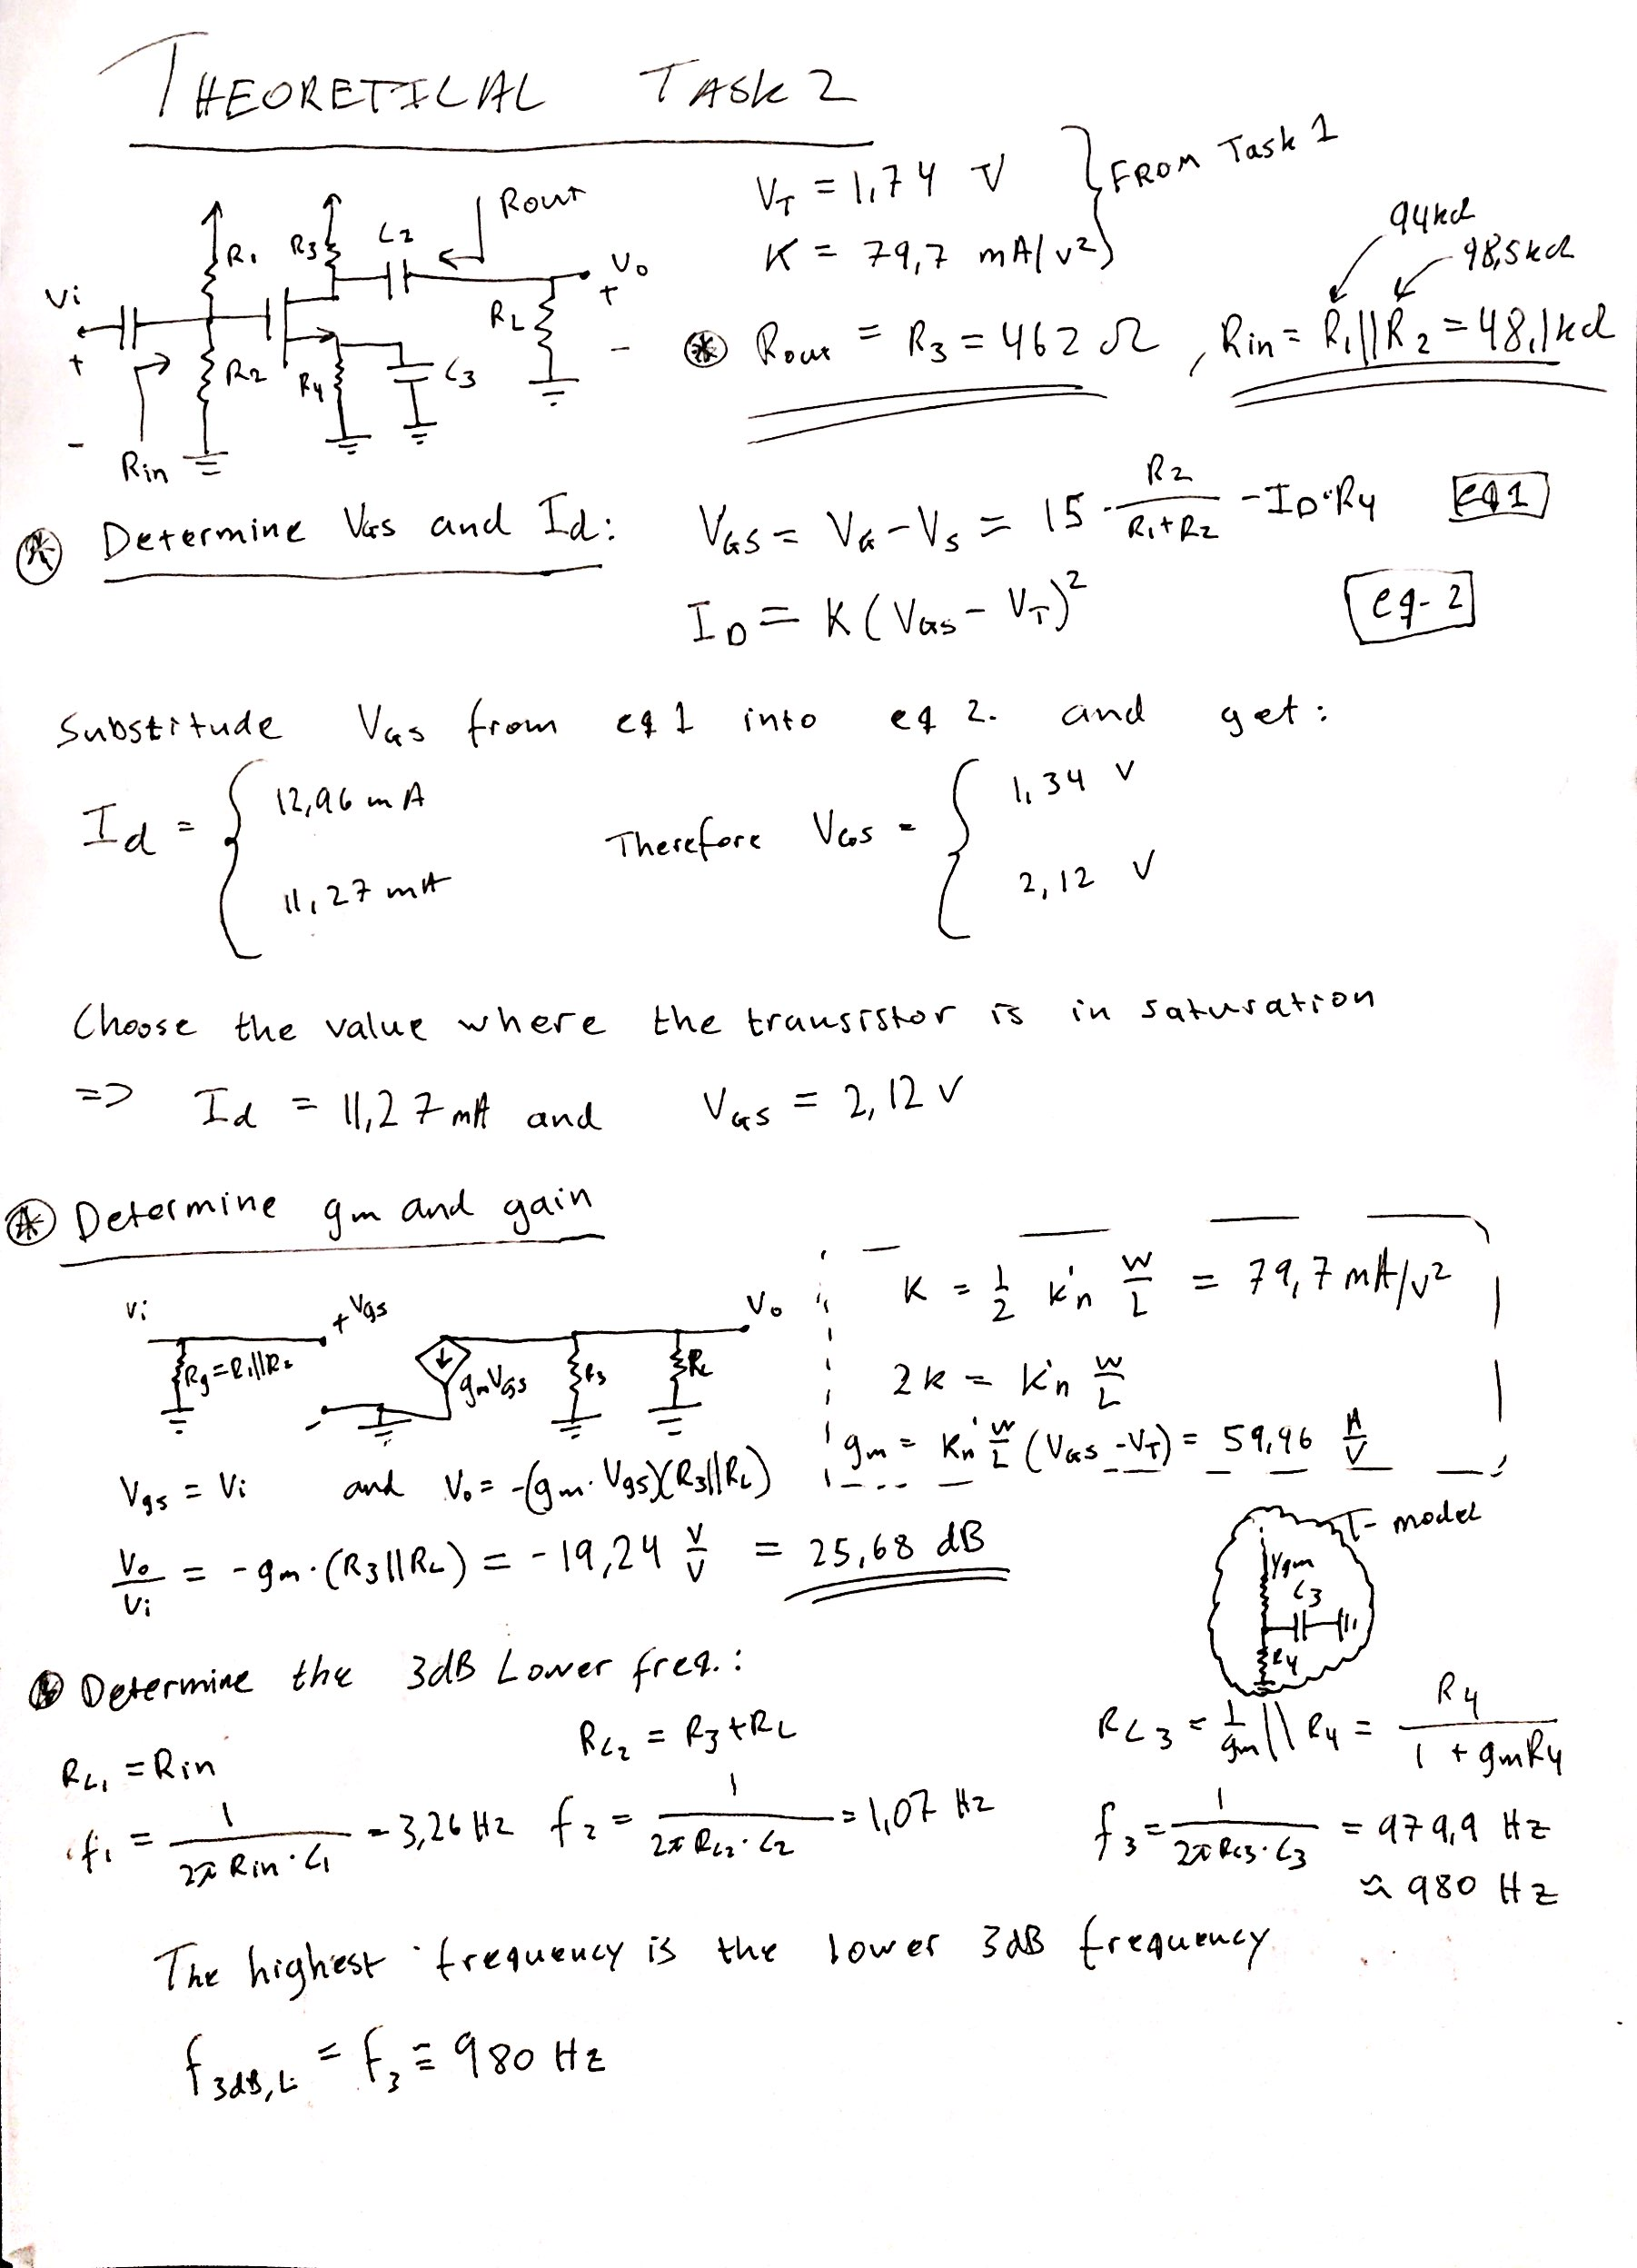
\includegraphics[scale = 0.29]{theoretical_task2_1.jpg}
\end{figure}
